\documentclass[border=10pt]{standalone}
\usepackage{tikz,amsmath}
\usetikzlibrary{arrows.meta,positioning,shapes.geometric,calc}

% ========== 配色方案（源色严格对应） ==========
\definecolor{c0Fill}{RGB}{183,224,177}
\definecolor{c0Line}{RGB}{32,102,32}
\definecolor{c1Fill}{RGB}{214,228,250}
\definecolor{c1Line}{RGB}{60,90,170}
\definecolor{c2Fill}{RGB}{250,224,180}
\definecolor{c2Line}{RGB}{190,110,20}
\definecolor{c3Fill}{RGB}{199,203,243}
\definecolor{c3Line}{RGB}{52,58,143}
\definecolor{c4Fill}{RGB}{243,199,199}
\definecolor{c4Line}{RGB}{143,52,52}
\definecolor{opFill}{RGB}{250,250,250}
\definecolor{opLine}{RGB}{70,70,70}
\definecolor{convFill}{RGB}{240,243,248}
\definecolor{convLine}{RGB}{70,85,110}

\begin{document}
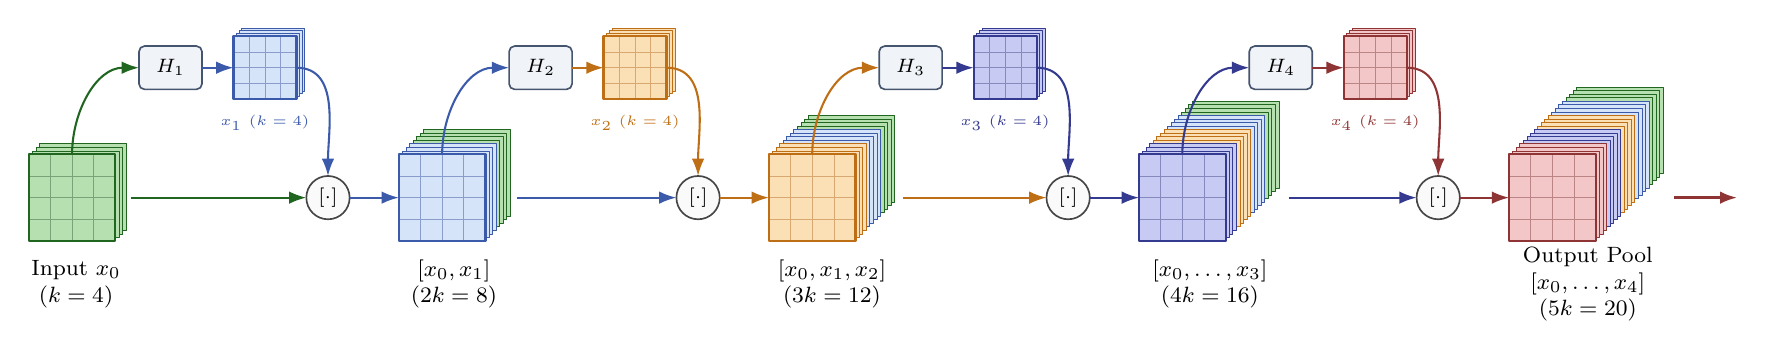
\begin{tikzpicture}[
    font=\small, line join=round,
    every node/.style={inner sep=0pt, outer sep=0pt, align=center},
    >={Latex[length=2.2mm, width=1.6mm]},
    arr/.style={->, line width=.75pt},
    concat/.style={circle, draw=opLine, fill=opFill, minimum size=.55cm, line width=.6pt, font=\scriptsize},
    conv/.style={rectangle, draw=convLine, fill=convFill, rounded corners=2pt, minimum width=.8cm, minimum height=.55cm, font=\scriptsize\bfseries, line width=.6pt}
  ]

  % 宏 1：绘制单层输出切片（固定 k=4 个特征图）
  % 参数: #1=X坐标, #2=Y坐标, #3=层颜色ID(0..4), #4=边长, #5=片间偏移
  \newcommand{\singlek}[5]{%
    \foreach \s in {3,...,0}{%
      \ifcase#3 \def\cc{c0}\or\def\cc{c1}\or\def\cc{c2}\or\def\cc{c3}\or\def\cc{c4}\fi
      \ifnum\s=0
        \fill[\cc Fill] ({#1},{#2}) rectangle ++(#4,#4);
        \draw[step={#4/4}, \cc Line!60, line width=.25pt, shift={({#1},{#2})}] (0,0) grid (#4,#4);
        \draw[\cc Line, thick] ({#1},{#2}) rectangle ++(#4,#4);
      \else
        \fill[\cc Fill, draw=\cc Line, line width=.2pt]
              ({#1+#5*\s},{#2+#5*\s}) rectangle ++(#4,#4);
      \fi
    }%
  }

  % 宏 2：绘制主干通道累积特征池 [x0, ..., xl]（包含所有前驱层切片）
  % 参数: #1=X坐标, #2=Y坐标, #3=包含的最大层号(0..4), #4=边长, #5=片间偏移
  \newcommand{\poolstack}[5]{%
    \pgfmathtruncatemacro{\totSlices}{4*(#3+1)-1}
    \foreach \s in {\totSlices,...,0}{%
      \pgfmathtruncatemacro{\ci}{#3-int(\s/4)}
      \ifcase\ci \def\cc{c0}\or\def\cc{c1}\or\def\cc{c2}\or\def\cc{c3}\or\def\cc{c4}\fi
      \ifnum\s=0
        \fill[\cc Fill] ({#1},{#2}) rectangle ++(#4,#4);
        \draw[step={#4/4}, \cc Line!60, line width=.25pt, shift={({#1},{#2})}] (0,0) grid (#4,#4);
        \draw[\cc Line, thick] ({#1},{#2}) rectangle ++(#4,#4);
      \else
        \fill[\cc Fill, draw=\cc Line, line width=.2pt]
              ({#1+#5*\s},{#2+#5*\s}) rectangle ++(#4,#4);
      \fi
    }%
  }

  % 尺寸控制变量
  \def\w{1.1}
  \def\off{0.045}

  % 上移高度控制：H 节点高度 \hy，支路特征图高度 \fy
  \def\hy{1.65}
  \def\fy{1.25}

  % ==================== Stage 0: Input x0 ====================
  \poolstack{-7.5}{-0.55}{0}{\w}{\off}
  \node at (-6.9, -1.1) [font=\footnotesize] {Input $x_0$\\($k=4$)};

  % H1 卷积支路（从第 1 张特征图正上方 (-6.95, 0.55) 引出）
  \node[conv] (h1) at (-5.7, \hy) {$H_1$};
  \draw[arr, c0Line] (-6.95, 0.55) to[out=90, in=180] (h1.west);
  \singlek{-4.9}{\fy}{1}{0.8}{0.035}
  \node at (-4.5, \fy-0.3) [font=\tiny, text=c1Line] {$x_1$ ($k=4$)};
  \draw[arr, c1Line] (h1.east) -- (-4.9, \hy);

  % Concat 1：从第一张特征图右边缘中点 (-4.1, \fy+0.4) 引出
  \node[concat] (cc1) at (-3.7, 0) {$[\cdot]$};
  \draw[arr, c0Line] (-6.2, 0) -- (cc1.west);
  \draw[arr, c1Line] (-4.1, \fy+0.4) to[out=0, in=90] (cc1.north);

  % ==================== Stage 1: Pool [x0, x1] ====================
  \poolstack{-2.8}{-0.55}{1}{\w}{\off}
  \draw[arr, c1Line] (cc1.east) -- (-2.8, 0);
  \node at (-2.1, -1.1) [font=\footnotesize] {$[x_0, x_1]$\\($2k=8$)};

  % H2 卷积支路（从第 1 张特征图正上方 (-2.25, 0.55) 引出）
  \node[conv] (h2) at (-1.0, \hy) {$H_2$};
  \draw[arr, c1Line] (-2.25, 0.55) to[out=90, in=180] (h2.west);
  \singlek{-0.2}{\fy}{2}{0.8}{0.035}
  \node at (0.2, \fy-0.3) [font=\tiny, text=c2Line] {$x_2$ ($k=4$)};
  \draw[arr, c2Line] (h2.east) -- (-0.2, \hy);

  % Concat 2：从第一张特征图右边缘中点 (0.6, \fy+0.4) 引出
  \node[concat] (cc2) at (1.0, 0) {$[\cdot]$};
  \draw[arr, c1Line] (-1.3, 0) -- (cc2.west);
  \draw[arr, c2Line] (0.6, \fy+0.4) to[out=0, in=90] (cc2.north);

  % ==================== Stage 2: Pool [x0, x1, x2] ====================
  \poolstack{1.9}{-0.55}{2}{\w}{\off}
  \draw[arr, c2Line] (cc2.east) -- (1.9, 0);
  \node at (2.7, -1.1) [font=\footnotesize] {$[x_0, x_1, x_2]$\\($3k=12$)};

  % H3 卷积支路（从第 1 张特征图正上方 (2.45, 0.55) 引出）
  \node[conv] (h3) at (3.7, \hy) {$H_3$};
  \draw[arr, c2Line] (2.45, 0.55) to[out=90, in=180] (h3.west);
  \singlek{4.5}{\fy}{3}{0.8}{0.035}
  \node at (4.9, \fy-0.3) [font=\tiny, text=c3Line] {$x_3$ ($k=4$)};
  \draw[arr, c3Line] (h3.east) -- (4.5, \hy);

  % Concat 3：从第一张特征图右边缘中点 (5.3, \fy+0.4) 引出
  \node[concat] (cc3) at (5.7, 0) {$[\cdot]$};
  \draw[arr, c2Line] (3.6, 0) -- (cc3.west);
  \draw[arr, c3Line] (5.3, \fy+0.4) to[out=0, in=90] (cc3.north);

  % ==================== Stage 3: Pool [x0, x1, x2, x3] ====================
  \poolstack{6.6}{-0.55}{3}{\w}{\off}
  \draw[arr, c3Line] (cc3.east) -- (6.6, 0);
  \node at (7.5, -1.1) [font=\footnotesize] {$[x_0,\dots,x_3]$\\($4k=16$)};

  % H4 卷积支路（从第 1 张特征图正上方 (7.15, 0.55) 引出）
  \node[conv] (h4) at (8.4, \hy) {$H_4$};
  \draw[arr, c3Line] (7.15, 0.55) to[out=90, in=180] (h4.west);
  \singlek{9.2}{\fy}{4}{0.8}{0.035}
  \node at (9.6, \fy-0.3) [font=\tiny, text=c4Line] {$x_4$ ($k=4$)};
  \draw[arr, c4Line] (h4.east) -- (9.2, \hy);

  % Concat 4：从第一张特征图右边缘中点 (10.0, \fy+0.4) 引出
  \node[concat] (cc4) at (10.4, 0) {$[\cdot]$};
  \draw[arr, c3Line] (8.5, 0) -- (cc4.west);
  \draw[arr, c4Line] (10.0, \fy+0.4) to[out=0, in=90] (cc4.north);

  % ==================== Stage 4: Output Pool ====================
  \poolstack{11.3}{-0.55}{4}{\w}{\off}
  \draw[arr, c4Line] (cc4.east) -- (11.3, 0);
  \node at (12.3, -1.1) [font=\footnotesize] {Output Pool\\$[x_0,\dots,x_4]$\\($5k=20$)};
  
  \draw[arr, c4Line, very thick] (13.4, 0) -- (14.2, 0);

\end{tikzpicture}
\end{document}